\chapter{RIP Tests Generator}
\label{chapter3}

\section{Solución propuesta}
Como fue mencionado anteriormente, uno de los principales problemas a la hora de generar casos de prueba, es poder tener en cuenta los diferentes cambios de contexto y los tipos de entidades encontrados en la aplicación. Por esto, la generación de tests de esta herramienta está basada en los diferentes modelos encontrados con la herramienta  \textbf{RIP}\cite{LinanAutomatedApps}. Concretamente se tienen definidos tres modelos: GUI, contexto y dominio, los cuales se basan en lo propuesto en CEL\cite{Linares-Vasquez2017ContinuousTesting}.

El modelo GUI es extraído mediante la técnica GUI ripping, en donde se realiza una exploración de la interfaz de la aplicación, generando un diagrama de estados que representan las actividades y eventos de transición entre ellas. Para el modelo de dominio, se realiza un análisis de los componentes encontrados en los XML's de la aplicación, para así describir los datos que pueden ser introducidos o producidos. Finalmente, mediante el diagrama de contexto se conocen las condiciones externas que podrían afectar el correcto funcionamiento de la aplicación. Información como sensores,  uso de batería, o conectividad es recolectada en este modelo.

Una vez se tiene la información sobre los diversos modelos, se propone crear \textbf{RIP Tests Generator}, una herramienta que genere de manera automática los archivos de prueba usando Espresso. Este es el framework sugerido por Google con el fin de escribir pruebas de para aplicaciones Android.



\section{Arquitectura de la solución}

\textbf{RIP Tests Generator} genera tests después de que \textbf{RIP} termina la ejecución, lo que permite el desacoplamiento de las dos herramientas. En este caso, \textbf{RIP} \cite{LinanAutomatedApps} puede mejorar o cambiar sus algoritmos de exploración dinámica sobre aplicaciones móviles, manteniendo la compatibilidad con \textbf{RIP Tests Generator}. La figura \ref{procesoTests} presenta el resumen del proceso de generación de tests a partir de los archivos obtenidos mediante la ejecución de RIP.

\begin{figure}[h]
	\centering
	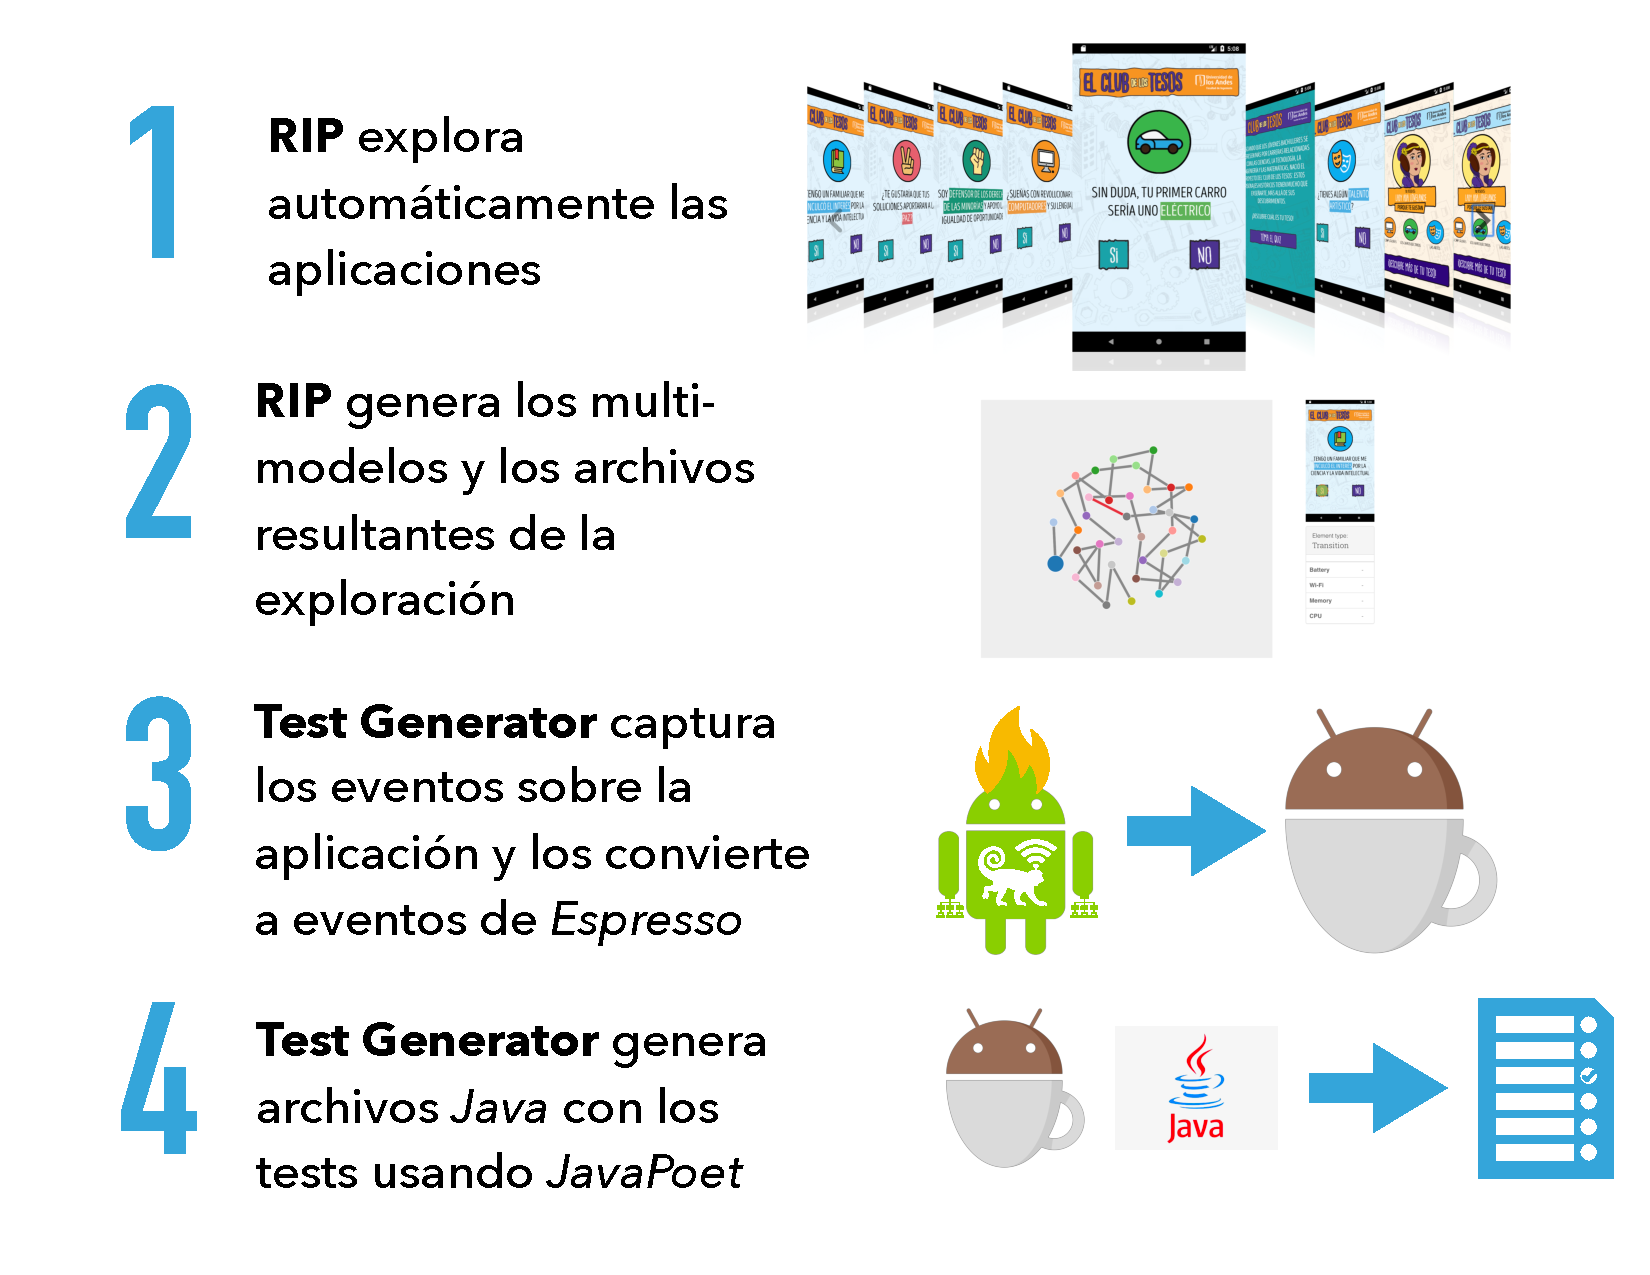
\includegraphics[width=1\textwidth]{img/procesoTests.pdf}
	\vspace{-0.5cm}
	\caption{Proceso de generación automática de tests}
	\label{procesoTests}
\end{figure} 

Test Generator es un componente acoplado con RIP que es ejecutado cuando se termina la exploración de la aplicación. Para esto, se creó la clase TestCaseBuilder.java que toma los datos proporcionados en el archivo tree.json y traduce los eventos a comandos de espresso.


Para la generación de pruebas se definieron los siguientes eventos, basados en los generados por RIP:

\textbf{TAP} : Cuando se tiene esta acción se traduce a un evento de hacer click en el botón o campo con el id proporcionado. Para implementar esta acción en espresso, se utiliza el comando \textit{onView(withId(id)).perform(click())}.

\textbf{INPUT} :  Al detectar un evento de campo de texto, con ayuda del modelo de dominio se detecta el tipo de dato a ingresar. Para esto se tiene la posibilidad de crear texto de manera aleatoria en un rango de caracteres normal o con una gran cantidad de estos con el fin de probar los limites de estos campos. Esta acción es implementada mediante el comando \textit{onView(withId(id)).perform(replaceText("randomtext"),closeSoftKeyboard());}



\section{Requisitos técnicos para la generación automática de pruebas}
Con el fin de que el desarrollador no tenga ningún inconveniente usando la herramienta, se definieron los siguientes requisitos técnicos:
\begin{enumerate}
	\item Al estar integrada con \textbf{RIP}\cite{LinanAutomatedApps}, se debe tener instalado ADB y correr el software en dispositivos rooteados o emuladores.
	\item El desarrollador debe tener acceso al código fuente de la aplicación, ya que los archivos de prueba generados solo pueden ser ejecutados si son empaquetados junto al código fuente.
	\item Es necesario htreeacer los cambios pertinentes en el build.gradle del proyecto para importar las dependencias utilizadas en los casos de prueba. Un ejemplo de esto es encontrado en la figura \ref{dependencies}.
	

\end{enumerate} 

	\begin{figure}[h]
	\centering
	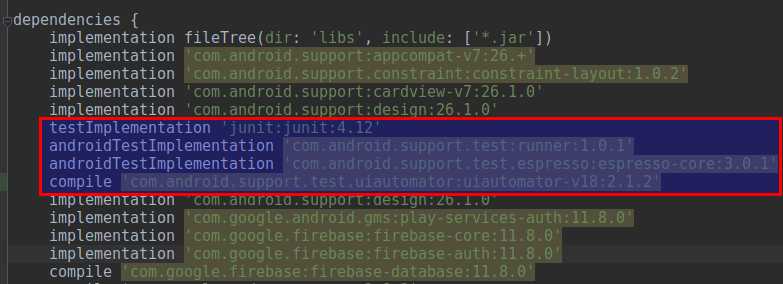
\includegraphics[width=1\textwidth]{img/dependencies.png}
	\vspace{-0.5cm}
	\caption{Ejemplo de archivo build.gradle con las dependencias necesarias para la ejecución de las pruebas}
	\label{dependencies}
\end{figure} 


\section{Generación automática de una prueba}
Para generar una prueba se hace uso del archivo tree.json \textbf{RIP}, el cual contiene un grafo donde las actividades corresponden a los nodos y los links a los eventos que disparan una transición entre dos estados. Cada nodo contiene la información del modelo de dominio con el tipo de datos que se encuentran. Además, se tienen los diferentes indicadores de contexto en cada estado, donde se pueden ver datos como batería, conectividad de internet, etc.

Dicho archivo es el que se utiliza como insumo para generar los casos de prueba mediante RIP Tests Generator. Gracias a la librería JavaPoet \cite{JavaPoet} se genera un archivo .java que contiene el código fuente de la prueba. Para esto, se tiene en cuenta la información obtenida del grafo generado por RIP y se hace una traducción de cada acción a ser ejecutada en la prueba.

Mediante el modelo GUI se pueden generar los eventos de transición. Por ejemplo, si la acción que produjo un cambio de estado es un tap en el botón con id 'buttonJugar', entonces esto será traducido como un \textit{onView(withId(R.id.buttonJugar)).perform(click());}. Para generar esto, se tiene un método auxiliar que retorna la línea de código correspondiente. Al analizar el grafo, según el tipo de acción encontrada se genera una línea de código diferente. Este proceso se puede evidenciar en el ejemplo de la figura \ref{gentest}.

Respecto a la implementación de la generación de código con JavaPoet se debe mencionar que las librerías correctamente declaradas son importadas de manera automática en el archivo generado. Además, el paquete donde debe ser ubicado el archivo fuente se inserta de manera correcta. Finalmente, después de cada acción, se toma una captura de pantalla que será posteriormente extraída del dispositivo para generar el reporte de visualización web.

El algoritmo propuesto para la generación de la prueba es el siguiente:

\begin{enumerate}
	\item Tomar la secuencia de eventos generada por RIP y guardarlos en una lista.
	\item Realizar la acción de tomar una captura de pantalla antes de cada transición.
	\item Según cada evento generar la línea de código correspondiente en el lenguaje espresso.
	\item Si se tiene un cambio de contexto en el nodo, realizar la traducción correspondiente.
	\item Con la ayuda de JavaPoet, generar los campos usados por Espresso. Como lo son la ActivityTestRule, para indicar en que actividad iniciar la aplicación, y los permisos de escritura y lectura para las capturas de pantalla.
	\item Finalmente, para la correcta ejecución de la prueba, se genera un archivo ejecutable que se encarga de empaquetar el apk, correr las pruebas encontradas en el paquete test, y extraer las capturas de pantalla del dispositivo.
\end{enumerate}
Un ejemplo de la prueba obtenida como resultado puede ser evidenciado en la figura \ref{pruebaresultado}

\begin{figure}[h]
	\centering
	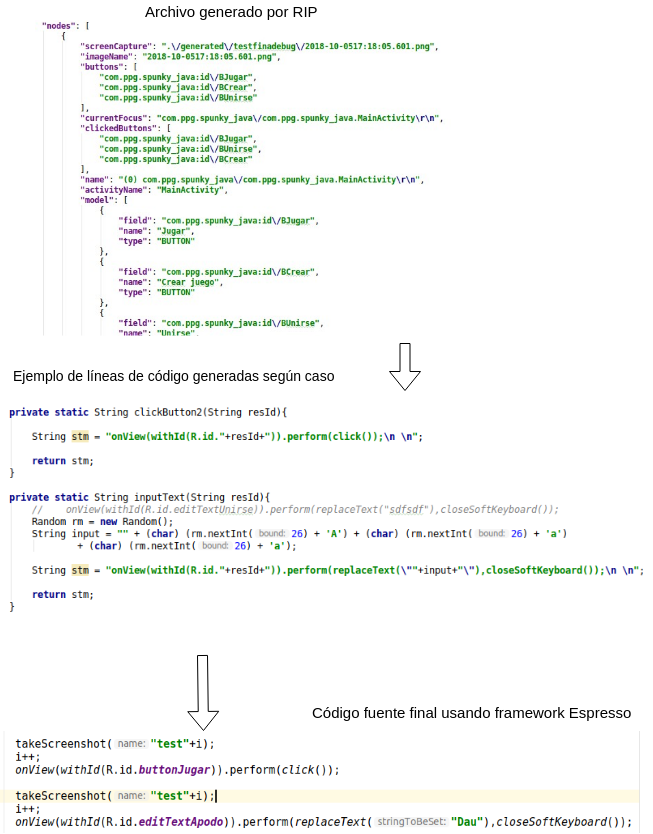
\includegraphics[width=1\textwidth]{img/GeneracionPrueba.png}
	\vspace{-0.5cm}
	\caption{Proceso de traducción y generación de prueba}
	\label{gentest}
\end{figure} 

\begin{figure}[h]
	\centering
	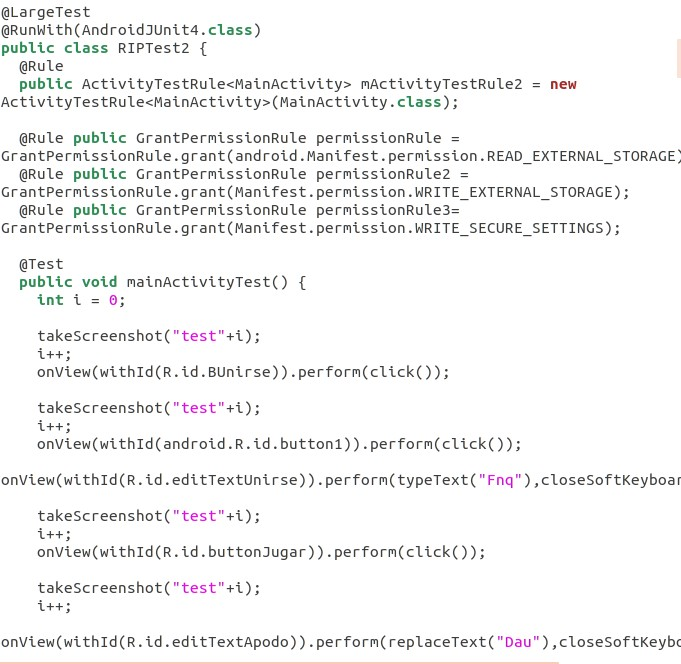
\includegraphics[width=1\textwidth]{img/pruebaResultado.jpg}
	\vspace{-0.5cm}
	\caption{Prueba generada}
	\label{pruebaresultado}
\end{figure} 







	
